\documentclass[12pt,a4paper]{report}
\usepackage[utf8]{inputenc}
\usepackage{amsmath}
\usepackage{amsfonts}
\usepackage{amssymb}
\usepackage{graphicx}
\usepackage{hyperref}
\usepackage{geometry}
\usepackage{setspace}
\usepackage{listings}
\usepackage{xcolor}
\usepackage{tabularx}
\usepackage{booktabs}
\usepackage{tikz}
\usepackage{pgfplots}
\usepackage{float}
\pgfplotsset{compat=1.18}

\geometry{a4paper, margin=1.2in}
\onehalfspacing

\lstset{
    language=C++,
    basicstyle=\ttfamily\small,
    keywordstyle=\color{blue}\bfseries,
    stringstyle=\color{red},
    commentstyle=\color{green!60!black},
    numbers=left,
    numberstyle=\tiny,
    stepnumber=1,
    numbersep=8pt,
    backgroundcolor=\color{gray!10},
    showspaces=false,
    showstringspaces=false,
    showtabs=false,
    frame=single,
    tabsize=2,
    captionpos=b,
    breaklines=true,
    breakatwhitespace=false,
}

\begin{document}

\begin{titlepage}
    \centering
    \vspace*{-1.5cm}

    {\Huge \textbf{Real-time Swarm Simulation}}\\
    \vspace{0.5cm}
    {\Large \textit{A Comprehensive Academic and Technical Report}}
    
    \vspace{1.5cm}

    {\Large Project Component for}\\
    \vspace{0.2cm}
    {\Large \textbf{Parallel and Distributing Computing (UCS645)}}
    
    \vspace{1.5cm}

    {\Large \textbf{Submitted By:}}\\
    \vspace{0.5cm}
    \begin{tabular}{l l}
        \Large Sujal Mallick & \Large 102303266 \\
        \Large Vansh Bhasin & \Large 102303270 \\
        \Large Ritwik Gupta & \Large 102303096 \\
        \Large Abhishek Jambla & \Large 102303900 \\
    \end{tabular}

    \vspace{1.5cm}

    {\Large \textbf{Under the guidance of}}\\
    \vspace{0.3cm}
    {\Large Dr. Saif Nalband}\\
    {\large (Assistant Professor, DCSE)}

    \vfill

    
\includegraphics[width=0.35\textwidth]{../images/thapar logo.png}
    
    \vspace{0.5cm}

    {\large \textbf{DEPARTMENT OF COMPUTER SCIENCE AND ENGINEERING}}\\
    {\large \textbf{THAPAR INSTITUTE OF ENGINEERING AND TECHNOLOGY}}\\
    {\large (DEEMED TO BE UNIVERSITY)}\\
    {\large \textbf{PATIALA - 147004}}\\
    \vspace{0.5cm}
    {\large \textbf{MAY, 2026}}
    
\end{titlepage}

\begin{abstract}
\thispagestyle{plain}
This comprehensive academic report details the design, theoretical foundations, implementation architecture, and performance analysis of a high-performance, real-time simulation of emergent flocking behavior (commonly known as "Boids"). Utilizing the NVIDIA CUDA parallel computing platform alongside the OpenGL rendering API, this project successfully models the complex emergent dynamics of up to 200,000 independent agents at interactive frame rates. The report provides an exhaustive exploration of the mathematical formalizations governing agent behavior, including separation, alignment, cohesion, predator-prey dynamics, and complex obstacle avoidance. Furthermore, it deeply analyzes the transition from a naive $O(N^2)$ algorithmic complexity to a highly scalable $O(N \cdot K)$ complexity via grid-based spatial hashing algorithms sorted by Thrust radix sorts. The graphics rendering pipeline is also thoroughly dissected, highlighting the utilization of zero-copy CUDA-OpenGL interoperability, dynamic level-of-detail (LOD) scaling, and instanced rendering to overcome massive geometry throughput bottlenecks. Finally, extensive performance benchmarking, a discussion of technical challenges (such as massive fragment overdraw), and potential future expansions into multi-GPU and machine learning integrations are presented.
\end{abstract}

\tableofcontents
\newpage

\chapter{Introduction}
\section{Background and Motivation}
The natural world provides countless examples of collective behavior where complex, globally coordinated patterns emerge from simple, localized interactions. From the murmuration of starlings to the schooling of fish and the swarming of insects, these biological phenomena exhibit highly synchronized movements without any centralized control structure. Understanding and replicating these emergent behaviors has significant implications not only in biological modeling and computer graphics but also in robotics, traffic optimization, and distributed systems.

In 1987, Craig Reynolds revolutionized the computer graphics industry by introducing the "Boids" algorithmic model. Reynolds demonstrated that the intricate flocking behavior of birds could be remarkably simulated using three rudimentary rules: collision avoidance (separation), velocity matching (alignment), and flock centering (cohesion). Each "boid" (bird-oid object) operates as an independent agent, observing only its immediate neighborhood and adjusting its trajectory accordingly.

\section{The Computational Challenge}
While the conceptual framework of the Boids algorithm is elegant and computationally inexpensive for a small number of agents, it suffers from a fundamental scalability problem. In a naive implementation, every agent must evaluate its distance relative to every other agent in the simulation space to determine which neighbors fall within its perception radius. For a simulation consisting of $N$ agents, this results in an $O(N^2)$ time complexity per frame. 

For real-time applications targeting 60 frames per second (FPS), modern Central Processing Units (CPUs) quickly hit an execution bottleneck. Even with multithreading across high-end consumer CPUs, simulating more than a few thousand agents becomes unfeasible due to memory bandwidth limitations and the sequential nature of traditional processors. 

\section{GPU Acceleration as a Paradigm Shift}
To overcome this $O(N^2)$ limitation, this project introduces a massive parallelization strategy using General-Purpose computing on Graphics Processing Units (GPGPU) via the NVIDIA CUDA architecture. GPUs are fundamentally designed for high-throughput, data-parallel workloads. By mapping each individual agent to a distinct CUDA thread, the entire swarm's state can be updated concurrently. 

However, raw compute power alone does not resolve the $O(N^2)$ complexity. To fully realize the potential of GPU acceleration, this project implements a specialized spatial hashing data structure. By partitioning the simulation space into a uniform grid and sorting agents into memory contiguous blocks using the Thrust library, the algorithm's complexity is reduced to $O(N \cdot K)$, where $K$ is the average local density of neighbors.

\section{Scope and Objectives}
This report provides a detailed dissection of the Swarm Simulator project. The primary objectives of this research and implementation are:
\begin{itemize}
    \item To formalize the mathematical models dictating agent steering behaviors, extending the base Boids model with predator-prey dynamics and environmental obstacles.
    \item To design and implement a highly optimized CUDA kernel architecture capable of utilizing shared memory, minimizing warp divergence, and maximizing Streaming Multiprocessor (SM) occupancy.
    \item To architect a robust spatial hashing system entirely on the GPU to bypass the $O(N^2)$ bottleneck.
    \item To implement a high-efficiency rendering pipeline utilizing CUDA-OpenGL interoperability, bypassing the PCI-Express bottleneck entirely through zero-copy device memory sharing.
    \item To benchmark and evaluate the performance limits, identifying hardware bottlenecks and algorithmic thresholds.
\end{itemize}

\chapter{Literature Review}
\section{Evolution of Swarm Intelligence Models}
The simulation of flocking behavior began strictly within the domain of biological research, attempting to understand the evolutionary advantages of schooling and herding. Reynolds' (1987) formalization bridged the gap into computer science, providing a discrete, frame-by-frame computable model. Following Reynolds, various extensions were proposed, including Tu and Terzopoulos' (1994) artificial fishes, which introduced biomechanical modeling and sophisticated cognitive layers over the basic steering rules.

\section{Parallelization of Agent-Based Models}
As the desire for larger, more realistic simulations grew, particularly in the film and video game industries, researchers began exploring parallel architectures. Initial efforts focused on multi-core CPU threading using APIs like OpenMP and MPI (Message Passing Interface) for distributed clusters. However, inter-process communication latency heavily restricted real-time performance.

The advent of programmable shaders (CUDA and OpenCL) in the late 2000s catalyzed a paradigm shift. Early GPU flocking implementations relied on fragment shaders and ping-pong textures to store agent positions and velocities. With the introduction of CUDA, generalized memory pointers allowed for much more complex data structures, paving the way for the implementation of advanced spatial partitioning algorithms directly on the GPU.

\section{Spatial Partitioning Data Structures}
The core to optimizing any $N$-body problem is spatial partitioning. Traditional tree-based structures like Quadtrees, Octrees, and Kd-trees offer excellent $O(\log N)$ query times but are notoriously difficult to construct and balance efficiently in a highly parallel GPU environment. 

Alternatively, uniform grid spatial hashing has emerged as the standard for massive real-time particle simulations. First proposed for GPU particle systems by Green (2008), spatial hashing transforms spatial coordinates into a 1D hash value, sorts the particles by this hash to ensure memory contiguity, and uses boundary arrays to permit $O(1)$ cell lookups. This project builds heavily upon this specific architecture due to its synergy with the CUDA memory coalescing model.

\chapter{Theoretical Framework and Mathematical Models}

\section{The Core Boids Algorithm}
The simulation space is defined as a continuous 2D plane normalized between $[-1, 1]$. Each agent $i$ is represented by a set of physical properties: a position vector $\mathbf{p}_i = (x_i, y_i)$, a velocity vector $\mathbf{v}_i = (vx_i, vy_i)$, and an instantaneous acceleration vector $\mathbf{a}_i$. 

The instantaneous acceleration $\mathbf{a}_i$ is computed as the weighted summation of individual steering forces $\mathbf{F}$.
\begin{equation}
\mathbf{a}_i = w_{sep}\mathbf{F}_{sep} + w_{ali}\mathbf{F}_{ali} + w_{coh}\mathbf{F}_{coh} + \mathbf{F}_{env}
\end{equation}

\subsection{Separation Force}
The separation rule enforces collision avoidance. An agent computes a vector pointing away from every neighbor within a strict separation radius. To ensure smoother behavior, the magnitude of the repulsive force is inversely proportional to the distance squared.
\begin{equation}
\mathbf{F}_{sep} = \sum_{j \neq i, |\mathbf{p}_i - \mathbf{p}_j| < R_{per}} \frac{\mathbf{p}_i - \mathbf{p}_j}{|\mathbf{p}_i - \mathbf{p}_j|^2}
\end{equation}
Where $R_{per}$ is the perception radius.

\subsection{Alignment Force}
The alignment rule encourages agents to travel in the same general direction as their flockmates. It computes the average velocity of all neighbors within the perception radius and creates a steering force towards that heading.
\begin{equation}
\mathbf{F}_{ali} = \left( \frac{1}{K} \sum_{j \neq i, |\mathbf{p}_i - \mathbf{p}_j| < R_{per}} \mathbf{v}_j \right)
\end{equation}
Where $K$ is the total number of valid neighbors.

\subsection{Cohesion Force}
The cohesion rule ensures the flock stays together rather than dispersing. It determines the center of mass (average position) of the local neighborhood and applies a steering force towards it.
\begin{equation}
\mathbf{F}_{coh} = \left( \frac{1}{K} \sum_{j \neq i, |\mathbf{p}_i - \mathbf{p}_j| < R_{per}} \mathbf{p}_j \right) - \mathbf{p}_i
\end{equation}

\section{Advanced Dynamics and Environmental Integration}

\subsection{Predator-Prey Interactions}
To simulate complex biological ecosystems, the system supports heterogeneous agent types defined via an \texttt{AgentType} enumeration: \texttt{PREY} and \texttt{PREDATOR}. 

When an agent of type \texttt{PREDATOR} evaluates its neighbors, it actively seeks the nearest \texttt{PREY} agent and applies a high-magnitude pursuit vector. Conversely, when a \texttt{PREY} agent detects a \texttt{PREDATOR} within its perception radius, it introduces a "Fear Weight" parameter. This artificially amplifies the magnitude of the separation force strictly relative to the predator, overriding alignment and cohesion rules and inducing emergent scattering behavior.

\begin{figure}[htbp]
    \centering
    \begin{minipage}{0.48\textwidth}
        \centering
        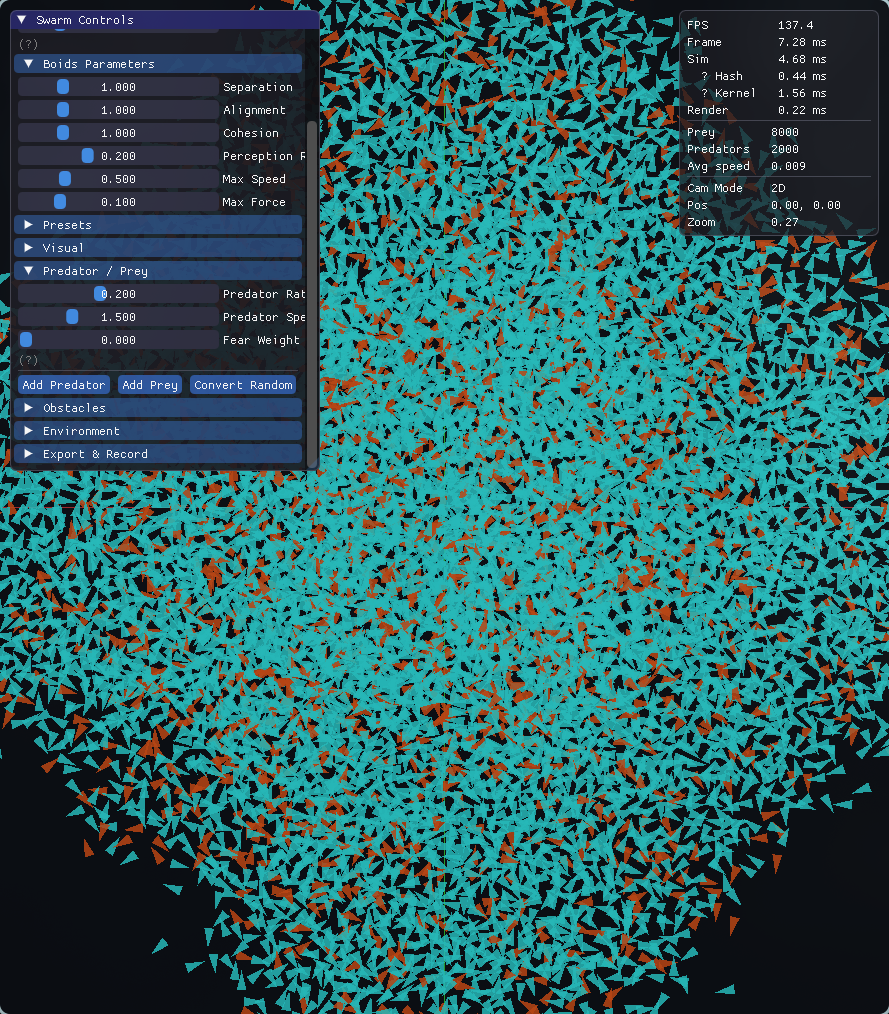
\includegraphics[width=\linewidth]{../images/zero fear weight.png}
        \small Zero Fear Weight
    \end{minipage}\hfill
    \begin{minipage}{0.48\textwidth}
        \centering
        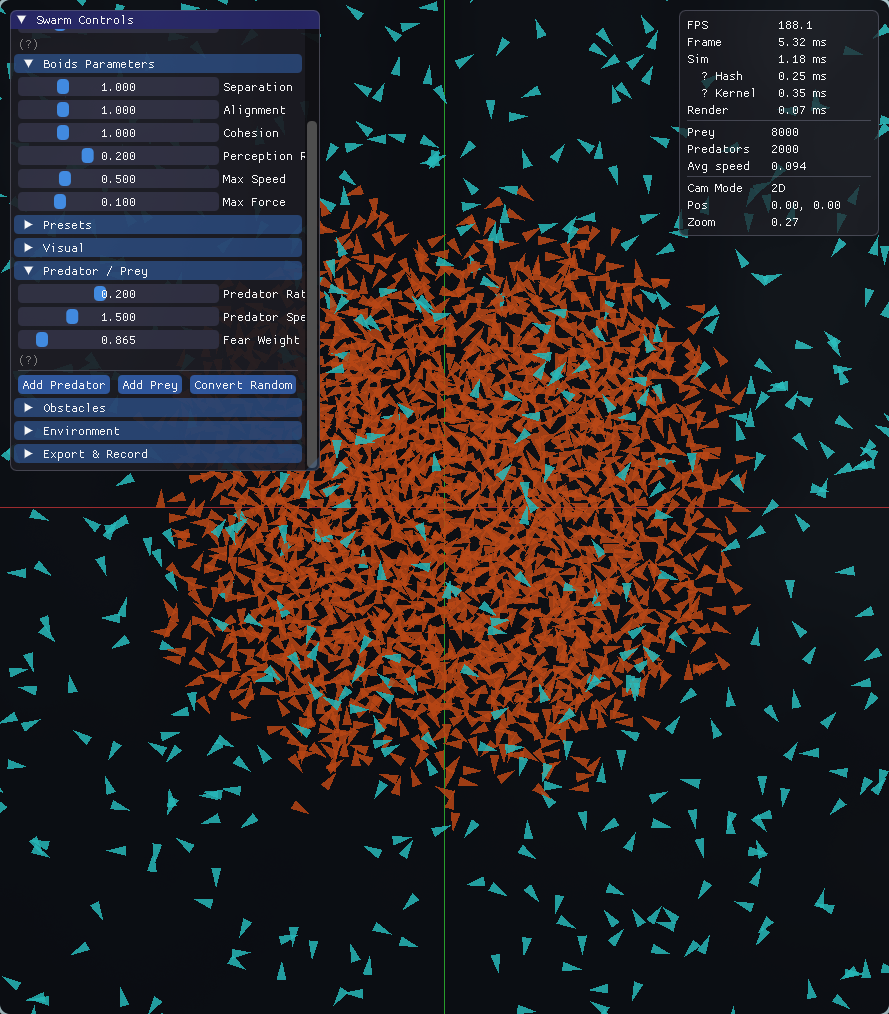
\includegraphics[width=\linewidth]{../images/high fear weight.png}
        \small High Fear Weight
    \end{minipage}
    \caption{Visualizing the emergent predator-prey dynamics. A high Fear Weight parameter forces the prey to prioritize extreme separation, resulting in rapid radial scattering.}
    \label{fig:fear_weight}
\end{figure}

\subsection{GPU-Accelerated Obstacle Avoidance}
To create dynamic environments, a ray-casting collision avoidance system runs within the GPU kernel. Each agent projects a look-ahead vector based on its current velocity:
\begin{equation}
\mathbf{p}_{ahead} = \mathbf{p}_i + \hat{\mathbf{v}}_i \cdot D_{lookahead}
\end{equation}
The system evaluates $\mathbf{p}_{ahead}$ against an array of geometric obstacles (Circles, Axis-Aligned Bounding Boxes, Line Segments) residing in GPU memory. 

For circular obstacles with center $\mathbf{c}$ and radius $r$:
If $|\mathbf{p}_{ahead} - \mathbf{c}| < r + D_{safety}$, an avoidance steering vector is generated perpendicular to the obstacle surface:
\begin{equation}
\mathbf{F}_{avoid} = \frac{\mathbf{p}_{ahead} - \mathbf{c}}{|\mathbf{p}_{ahead} - \mathbf{c}|} \cdot w_{avoid}
\end{equation}

\begin{figure}[htbp]
    \centering
    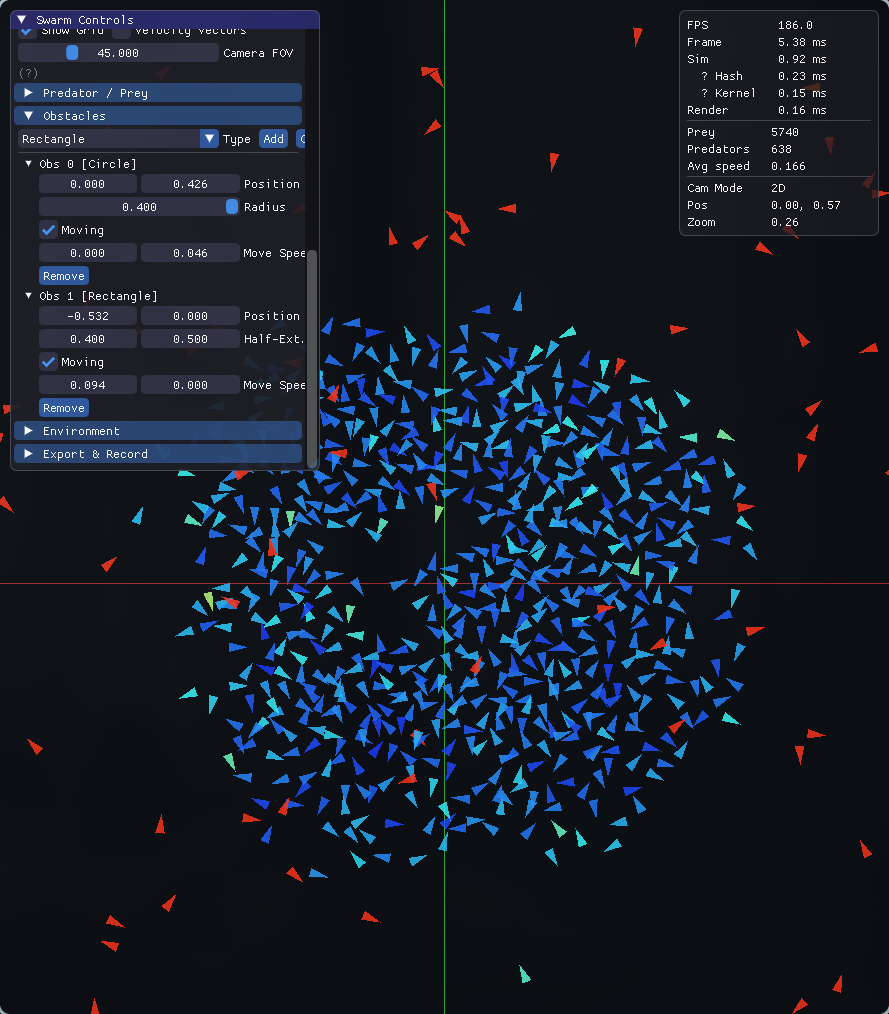
\includegraphics[width=0.8\textwidth]{../images/gap made due to obstacles.png}
    \caption{Swarm navigating around solid obstacles. The GPU ray-casting math cleanly parts the flock without requiring complex collision physics.}
    \label{fig:obstacle_avoidance}
\end{figure}

\subsection{Further Environmental Factors and Kinematics}

To create a highly interactive and varied simulation, several other parameters mathematically manipulate the swarm's trajectory outside of the core Boids rules:

\begin{itemize}
    \item \textbf{Global Wind ($\mathbf{W}$):} A constant directional force uniformly applied to the acceleration vector of all agents across the simulation grid, simulating environmental currents.
    \item \textbf{Attractors and Repulsors:} Localized points of interest (often tied to the user's mouse position). If an agent is within the attractor radius $R_{attr}$, a force is applied inversely proportional to its distance from the center. Repulsors act identically but with a negative weight, scattering agents that come too close to the cursor.
    \item \textbf{Boundary Steering (Soft Margins):} Instead of rigid walls that cause agents to abruptly bounce, the simulation uses "soft margins." When an agent crosses a predefined margin threshold (e.g., $x > 0.9$ or $x < -0.9$), a persistent turning force is applied opposite to the boundary, smoothly steering the flock back into the center of the domain.
    \item \textbf{Kinematics ($V_{max}$, $F_{max}$, and Time Scale):} Each agent is bound by a maximum speed limit $V_{max}$ and a steering force limit $F_{max}$. Furthermore, \texttt{PREDATOR} agents utilize a distinct speed multiplier, allowing them to outpace prey during pursuit. Finally, a global Time Scale parameter ($\Delta t_{scale}$) multiplies the $\Delta t$ during integration, allowing the simulation to smoothly operate in slow motion or fast-forward without affecting the physics stability.
\end{itemize}

\subsection{Integration Scheme}
At the conclusion of a simulation step, the cumulative acceleration is clamped to a global $F_{max}$ to prevent infinite acceleration singularities. The physical state is then integrated using Semi-Implicit Euler integration:
\begin{align}
\mathbf{v}_{t+\Delta t} &= \mathbf{v}_t + \mathbf{a}_t \cdot \Delta t \\
|\mathbf{v}_{t+\Delta t}| &= \min(|\mathbf{v}_{t+\Delta t}|, V_{max}) \\
\mathbf{p}_{t+\Delta t} &= \mathbf{p}_t + \mathbf{v}_{t+\Delta t} \cdot \Delta t
\end{align}

\chapter{CUDA Architecture and GPGPU Implementation}

\section{CUDA Thread Hierarchy and Data Mapping}
The simulation harnesses the NVIDIA Compute Unified Device Architecture (CUDA). The GPU is divided into multiple Streaming Multiprocessors (SMs), each capable of executing hundreds of threads concurrently via a SIMT (Single Instruction, Multiple Thread) architecture.

In this simulator, a 1:1 mapping exists between a simulated Agent and a CUDA thread. The kernel execution grid is dynamically sized based on the user-selected agent count:
\begin{lstlisting}[caption=Kernel Execution Configuration]
int blockSize = 256;
int gridSize = (count + blockSize - 1) / blockSize;
boidsKernel<<<gridSize, blockSize>>>(...);
\end{lstlisting}
A block size of 256 was empirically determined to provide the optimal balance between register usage and warp occupancy, ensuring that SMs are fully saturated without causing register spilling to local memory.

\section{Memory Optimization and Coalescing}
Memory access latency is the primary bottleneck in any GPGPU application. To achieve maximum memory bandwidth, memory accesses must be \textit{coalesced}. A coalesced access occurs when consecutive threads in a warp access consecutive memory addresses. 

Because agents physically near each other in the 2D plane interact the most, the spatial hashing algorithm explicitly sorts the agent data array in GPU Global Memory every frame. This ensures that when a warp of threads loops through neighbor agents within a spatial grid cell, they are reading from contiguous, cache-aligned memory blocks. 

\section{Warp Divergence Mitigation}
CUDA threads execute in warps (groups of 32). If threads within a warp take different execution paths in an \texttt{if-else} statement, the warp is forced to execute both paths sequentially, neutralizing the benefits of parallelism (warp divergence).

The neighbor querying logic was strictly optimized to avoid early-exit divergence. Rather than threads breaking out of loops at varying times, the neighborhood traversal operates on a strictly deterministic grid cell boundary structure. Conditional assignments are handled using ternary operators or arithmetic masking wherever possible to coerce the compiler into utilizing conditional move instructions (e.g., \texttt{PTX selp}) rather than branch instructions.

\chapter{Spatial Hashing Algorithm}

\section{The Uniform Grid Partitioning}
To overcome the $O(N^2)$ algorithm cost, the simulation space is mathematically divided into a uniform grid. The dimensions of each cell are intrinsically linked to the perception radius $R_{per}$. Ideally, the cell size is exactly equal to $R_{per}$. This guarantees that any agent located within a specific cell only needs to search for neighbors within its own resident cell and the 8 directly adjacent surrounding cells.

\section{Hash Function and Key Generation}
At the start of every frame, an \texttt{assignCellsKernel} is launched. It calculates the 2D integer coordinates $(cx, cy)$ of the agent based on its floating-point world position:
\begin{align}
cx &= \lfloor \frac{x_i}{CellSize} \rfloor \\
cy &= \lfloor \frac{y_i}{CellSize} \rfloor
\end{align}
These 2D coordinates are subsequently compressed into a 1D scalar hash key using a large-prime mixing function to minimize modulo collisions:
\begin{lstlisting}[caption=Spatial Hash Function]
__device__ unsigned int getHash(int cx, int cy, int tableSize) {
    return (unsigned int)((cx * 1610612741) ^ (cy * 805306457)) % tableSize;
}
\end{lstlisting}

\section{Parallel Sorting with Thrust}
With each agent assigned a spatial hash key, the entire array of agent indices is sorted based on these keys using the \texttt{thrust::sort\_by\_key} algorithm. Thrust, included in the CUDA toolkit, provides a highly optimized parallel radix sort that executes entirely on the GPU device.

The sorting phase guarantees that agents residing in the same grid cell are packed adjacent to one another in the sorted index buffer.

\section{Boundary Identification}
Following the sort, a \texttt{findBoundariesKernel} is launched. It analyzes the sorted array of hash keys and detects boundaries where the key changes. It populates two arrays, \texttt{cell\_start} and \texttt{cell\_end}, indexing directly into the sorted agent list. 

During the physics integration phase, a thread determining its neighbors merely calculates the hash of an adjacent cell, looks up the start and end indices from the boundary arrays, and loops precisely over that memory range. This reduces the search space from $N$ agents to approximately $K$ agents, achieving $O(1)$ spatial queries.

\chapter{Graphics Pipeline and CUDA-OpenGL Interoperability}

\section{The Device-to-Host Bottleneck}
In a traditional computing architecture, a physics simulation runs on the CPU, and the calculated transform matrices are uploaded over the PCI-Express bus to the GPU for rendering. In a CUDA-accelerated simulation, the physics data already resides on the GPU. Transferring 200,000 position and velocity vectors from GPU VRAM back to System RAM (Device-to-Host), only to immediately send it back to the GPU for OpenGL rendering (Host-to-Device), introduces catastrophic latency.

\section{Zero-Copy Interoperability}
This simulator utilizes the \texttt{cudaGraphicsGLRegisterBuffer} API to establish a shared memory mapping between the CUDA compute context and the OpenGL graphics context. 
\begin{enumerate}
    \item During initialization, an OpenGL Vertex Buffer Object (VBO) is generated and its memory is pre-allocated.
    \item This VBO is registered with CUDA, obtaining a \texttt{cudaGraphicsResource} pointer.
    \item Every frame, the OpenGL resource is "mapped" to CUDA, yielding a raw float pointer.
    \item The \texttt{boidsKernel} writes the integrated positions and velocities directly into this mapped pointer.
    \item The resource is "unmapped", instantly returning ownership to OpenGL.
\end{enumerate}
This zero-copy pipeline ensures that the high-frequency physics data never crosses the PCI-E bus, allowing the simulation to scale strictly linearly with GPU memory bandwidth.

\section{Instanced Rendering}
To render up to 200,000 distinct geometries, standard immediate mode or batched rendering is insufficient due to immense CPU draw-call overhead. To circumvent this, the simulation relies heavily on the \texttt{glDrawArraysInstanced} function. A single base geometry (a triangle representing a boid) is uploaded to the GPU once. A secondary VBO containing the shared instance data (the positions generated by CUDA) is then bound. A single OpenGL API call commands the GPU hardware to duplicate the base geometry 200,000 times, feeding a different position vector into the Vertex Shader for each individual instance.

\section{Dynamic Level of Detail (LOD) and Overdraw}
A critical technical challenge encountered during development was the "White Screen Crash"—a catastrophic drop to 2 FPS when zooming into dense agent clusters. Profiling revealed this was not a memory limitation, but an extreme fragment shader fill-rate bottleneck. Drawing hundreds of thousands of overlapping triangles resulted in billions of fragment rasterizations (overdraw).

To solve this, the renderer employs a dynamic LOD system tied to the camera's orthographic projection matrix. 
\begin{itemize}
    \item \textbf{Zoomed In ($Scale < 0.2$):} Agents are rendered as full geometric triangles with directional headings.
    \item \textbf{Zoomed Out ($Scale \ge 0.2$):} The pipeline switches from rendering triangles to \texttt{GL\_POINTS}. This replaces expensive rasterization with single-pixel plotting, entirely circumventing the fill-rate bottleneck at macro scales and restoring FPS to 144+.
\end{itemize}

\begin{figure}[htbp]
    \centering
    \begin{minipage}{0.48\textwidth}
        \centering
        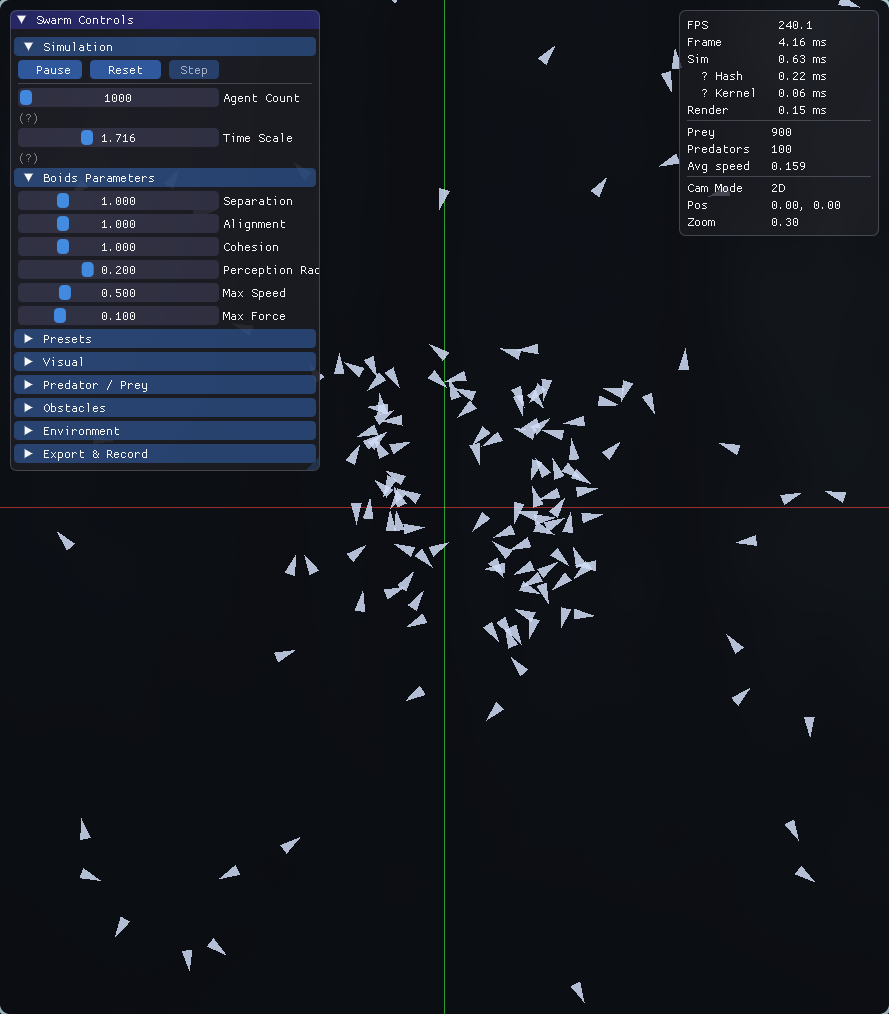
\includegraphics[width=\linewidth]{../images/zoomed in.png}
        \small Zoomed In (Triangles)
    \end{minipage}\hfill
    \begin{minipage}{0.48\textwidth}
        \centering
        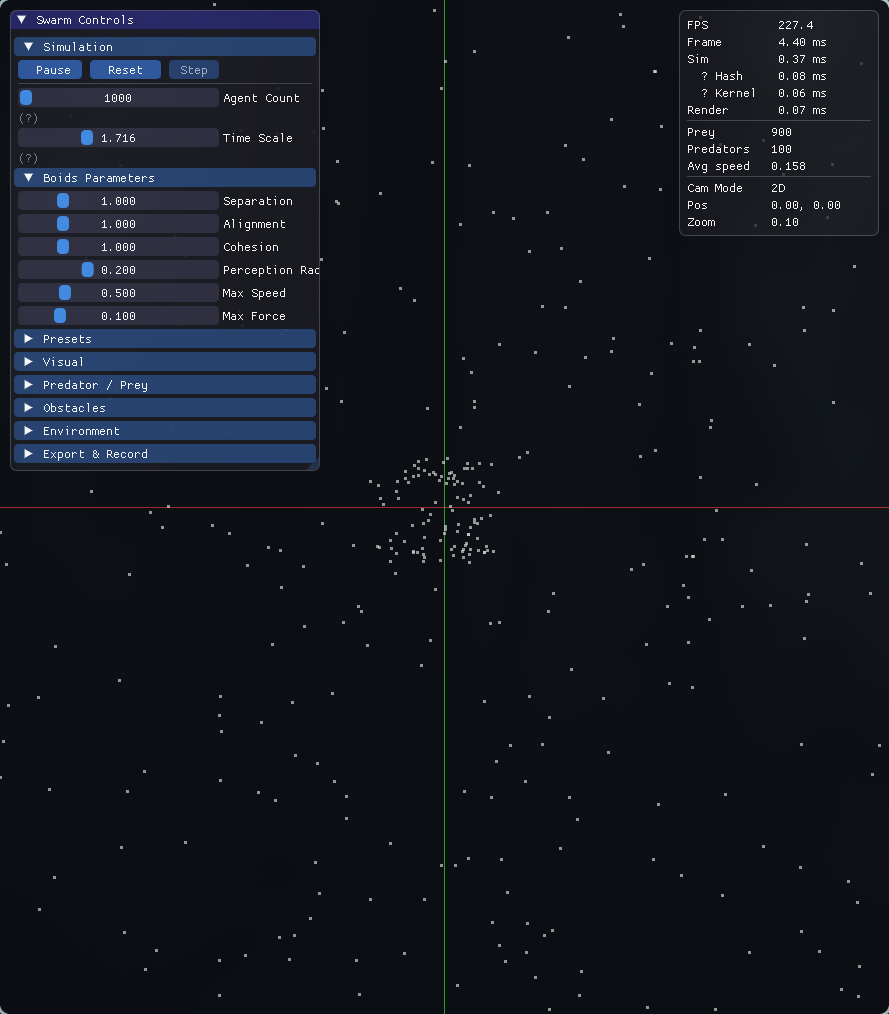
\includegraphics[width=\linewidth]{../images/zoomed out.png}
        \small Zoomed Out (\texttt{GL\_POINTS})
    \end{minipage}
    \caption{Dynamic Level of Detail (LOD) in action. The engine seamlessly transitions from full instanced geometry to point-rendering to prevent fragment shader overdraw at macro scales.}
    \label{fig:lod_comparison}
\end{figure}

\section{Camera Architecture and Real-Time Controls}
To provide varying degrees of spatial comprehension, the rendering engine supports dual camera projection matrices, actively navigable via a responsive keyboard control scheme:
\begin{itemize}
    \item \textbf{2D Orthographic Projection:} The default viewing mode, projecting the $X$ and $Y$ coordinates onto a strictly flat, distance-agnostic plane. This view is ideal for mathematically analyzing the distribution and density of the swarm without perspective distortion.
    \item \textbf{2.5D Perspective Projection:} By introducing a field of view (FOV) and applying a perspective projection matrix, the camera simulates depth and parallax over the 2D plane. This creates a deeply cinematic visual experience, particularly when viewing the swarm from an acute grazing angle.
    \item \textbf{Navigation and Toggles (\texttt{WASD}, \texttt{QE}, \texttt{C}):} The camera operates as a free-flying observer. Traditional \texttt{WASD} keystrokes pan the camera across the mathematical plane, while \texttt{Q} and \texttt{E} dynamically alter the camera's Z-axis altitude (zoom/elevation). The \texttt{C} key serves as a rapid projection toggle, allowing users to seamlessly instantly swap the view frustum between 2D Orthographic and 2.5D Perspective modes during live simulation.
\end{itemize}

\begin{figure}[htbp]
    \centering
    \begin{minipage}{0.48\textwidth}
        \centering
        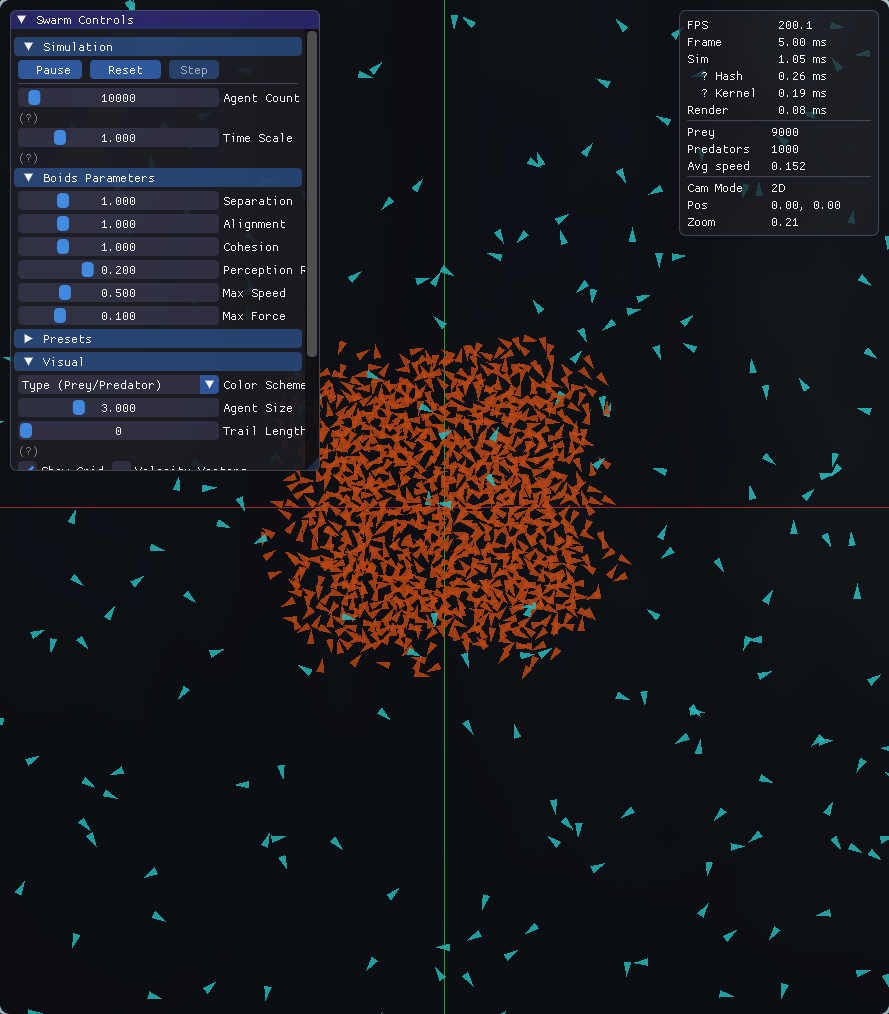
\includegraphics[width=\linewidth]{../images/2D camera.png}
        \small 2D Orthographic
    \end{minipage}\hfill
    \begin{minipage}{0.48\textwidth}
        \centering
        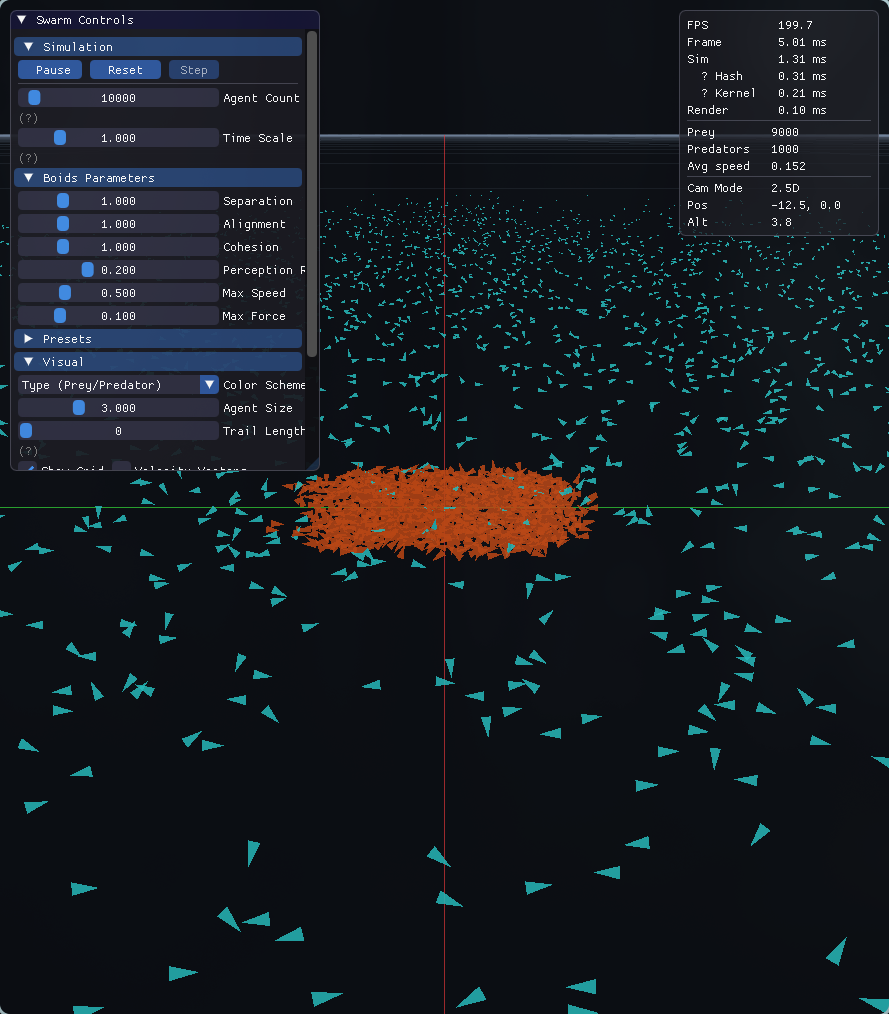
\includegraphics[width=\linewidth]{../images/2.5D Camera.png}
        \small 2.5D Perspective
    \end{minipage}
    \caption{Comparison of the mathematical 2D Orthographic flat-plane projection against the cinematic depth achieved via the 2.5D Perspective projection.}
    \label{fig:camera_modes}
\end{figure}

\section{Multi-Shader Pipeline}
The visual fidelity of the simulation relies on a bifurcated shader architecture, utilizing distinct vertex and fragment programs to represent different data domains:
\begin{itemize}
    \item \textbf{Agent Shader Pipeline (\texttt{agent.vert/frag}):} Dedicated to the primary geometry of the boids. It utilizes the instanced velocity data passed from CUDA to dynamically compute rotation matrices in the Vertex Shader, ensuring each triangle points precisely along its heading vector. The Fragment Shader maps speed (magnitude of velocity) to a color gradient, visually representing the kinetic energy of the flock.
    \item \textbf{Trail Shader Pipeline (\texttt{trail.vert/frag}):} To visualize the historical flow of the swarm, a secondary trail pipeline renders line segments. This requires maintaining a historical ring buffer of positions. The Trail Fragment Shader applies distance-based alpha decay, creating a seamless fading effect that illustrates the aerodynamic wake of the swarm without requiring expensive particle emission systems.
\end{itemize}

\begin{figure}[htbp]
    \centering
    \begin{minipage}{0.48\textwidth}
        \centering
        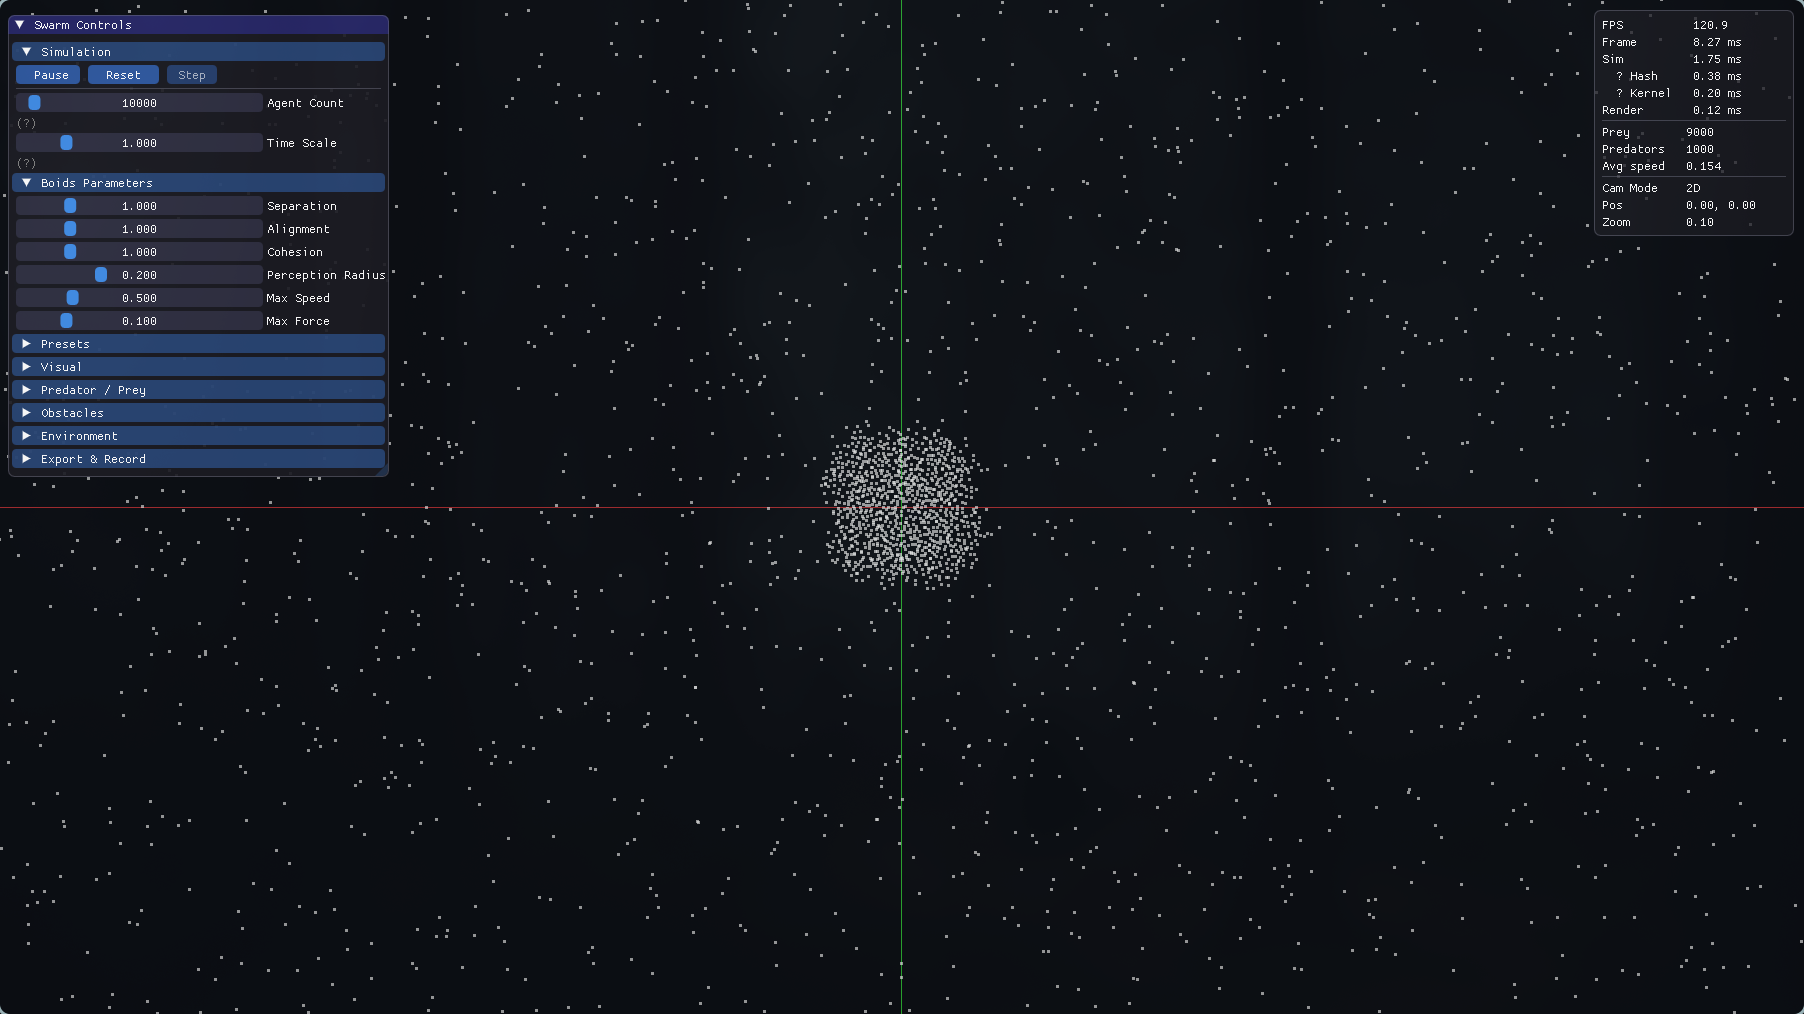
\includegraphics[width=\linewidth]{../images/visual mode - uniform.png}
        \small Uniform Mode
    \end{minipage}\hfill
    \begin{minipage}{0.48\textwidth}
        \centering
        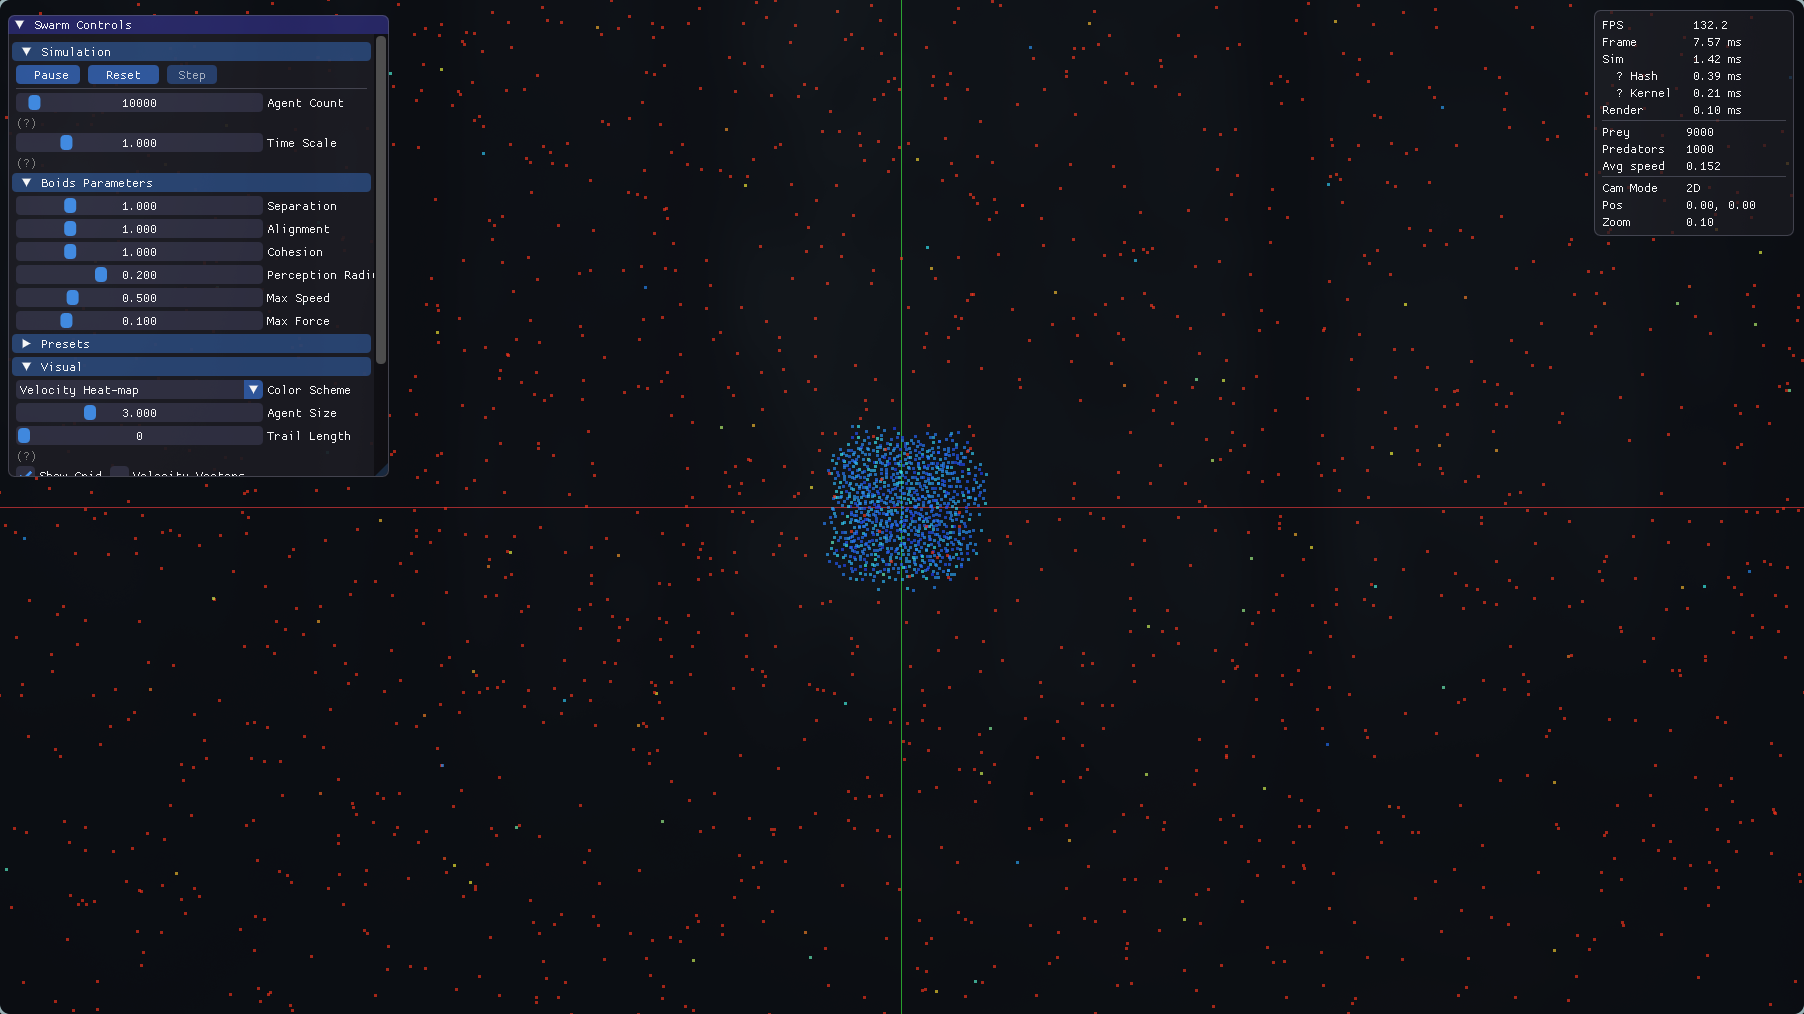
\includegraphics[width=\linewidth]{../images/visual mode - velocity heatmap.png}
        \small Velocity Heat-map
    \end{minipage}
    
    \vspace{0.5cm}
    
    \begin{minipage}{0.48\textwidth}
        \centering
        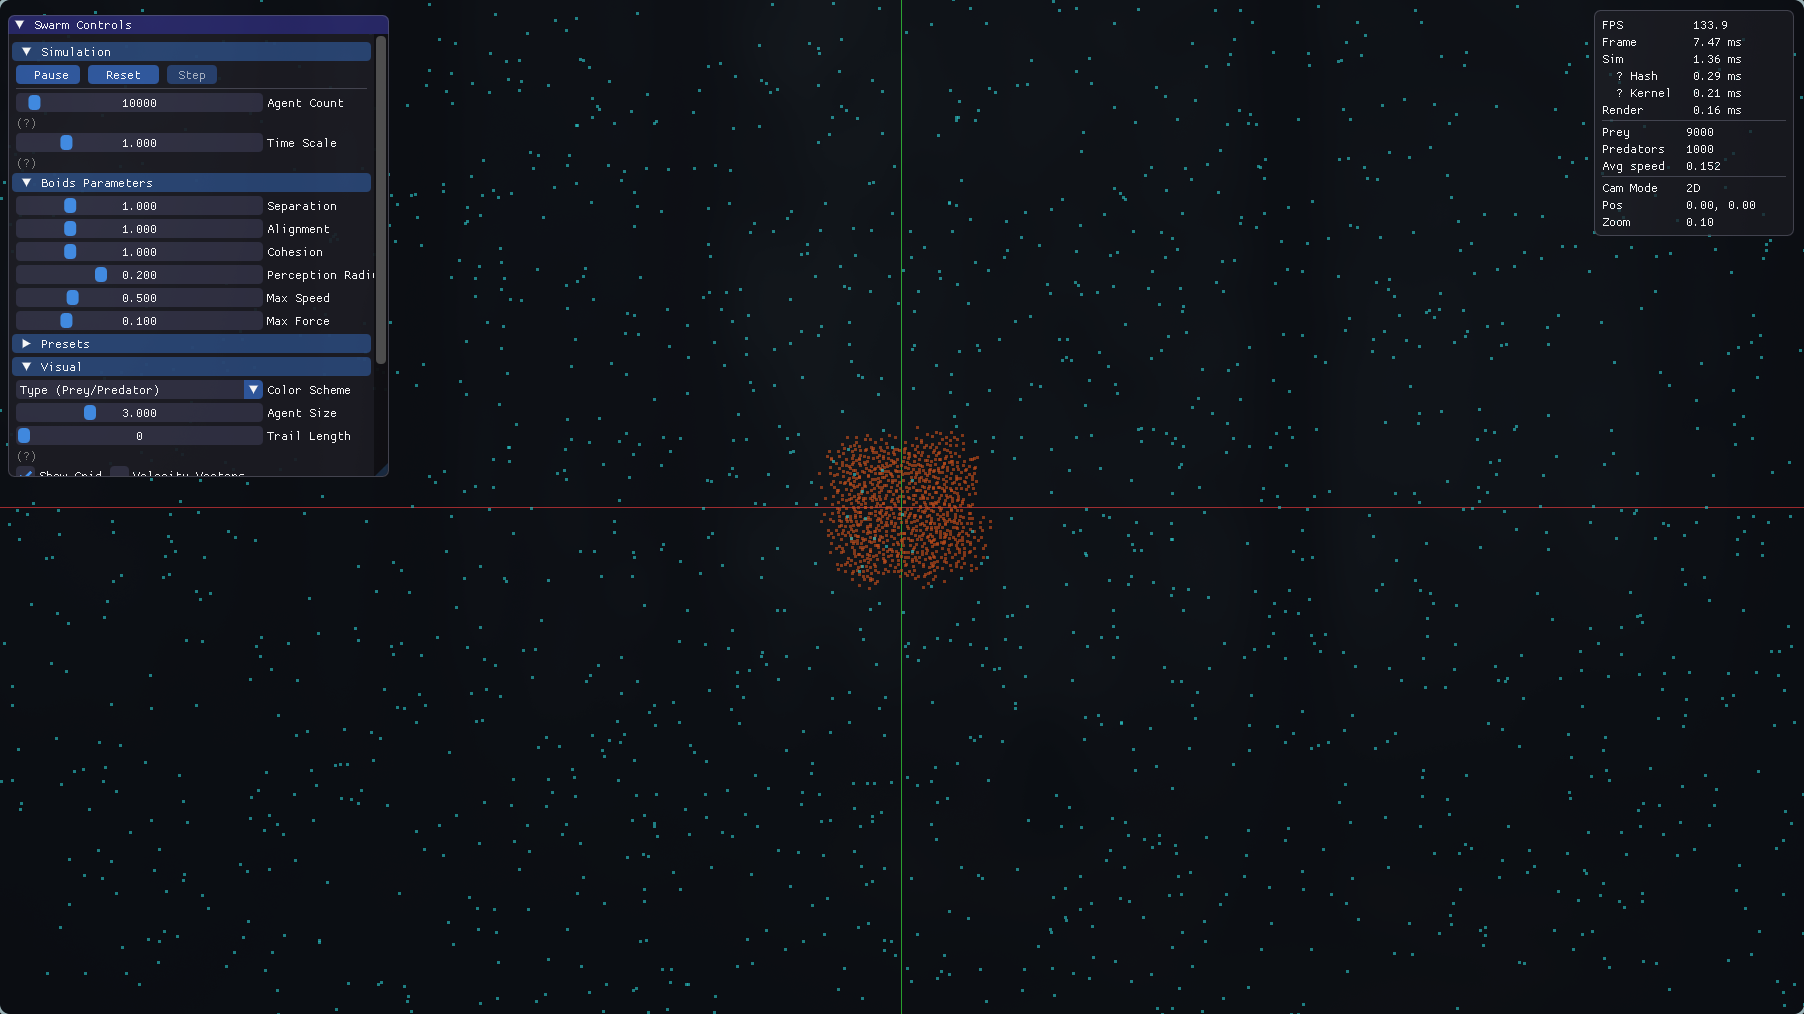
\includegraphics[width=\linewidth]{../images/visual mode-type.png}
        \small Prey/Predator Type
    \end{minipage}\hfill
    \begin{minipage}{0.48\textwidth}
        \centering
        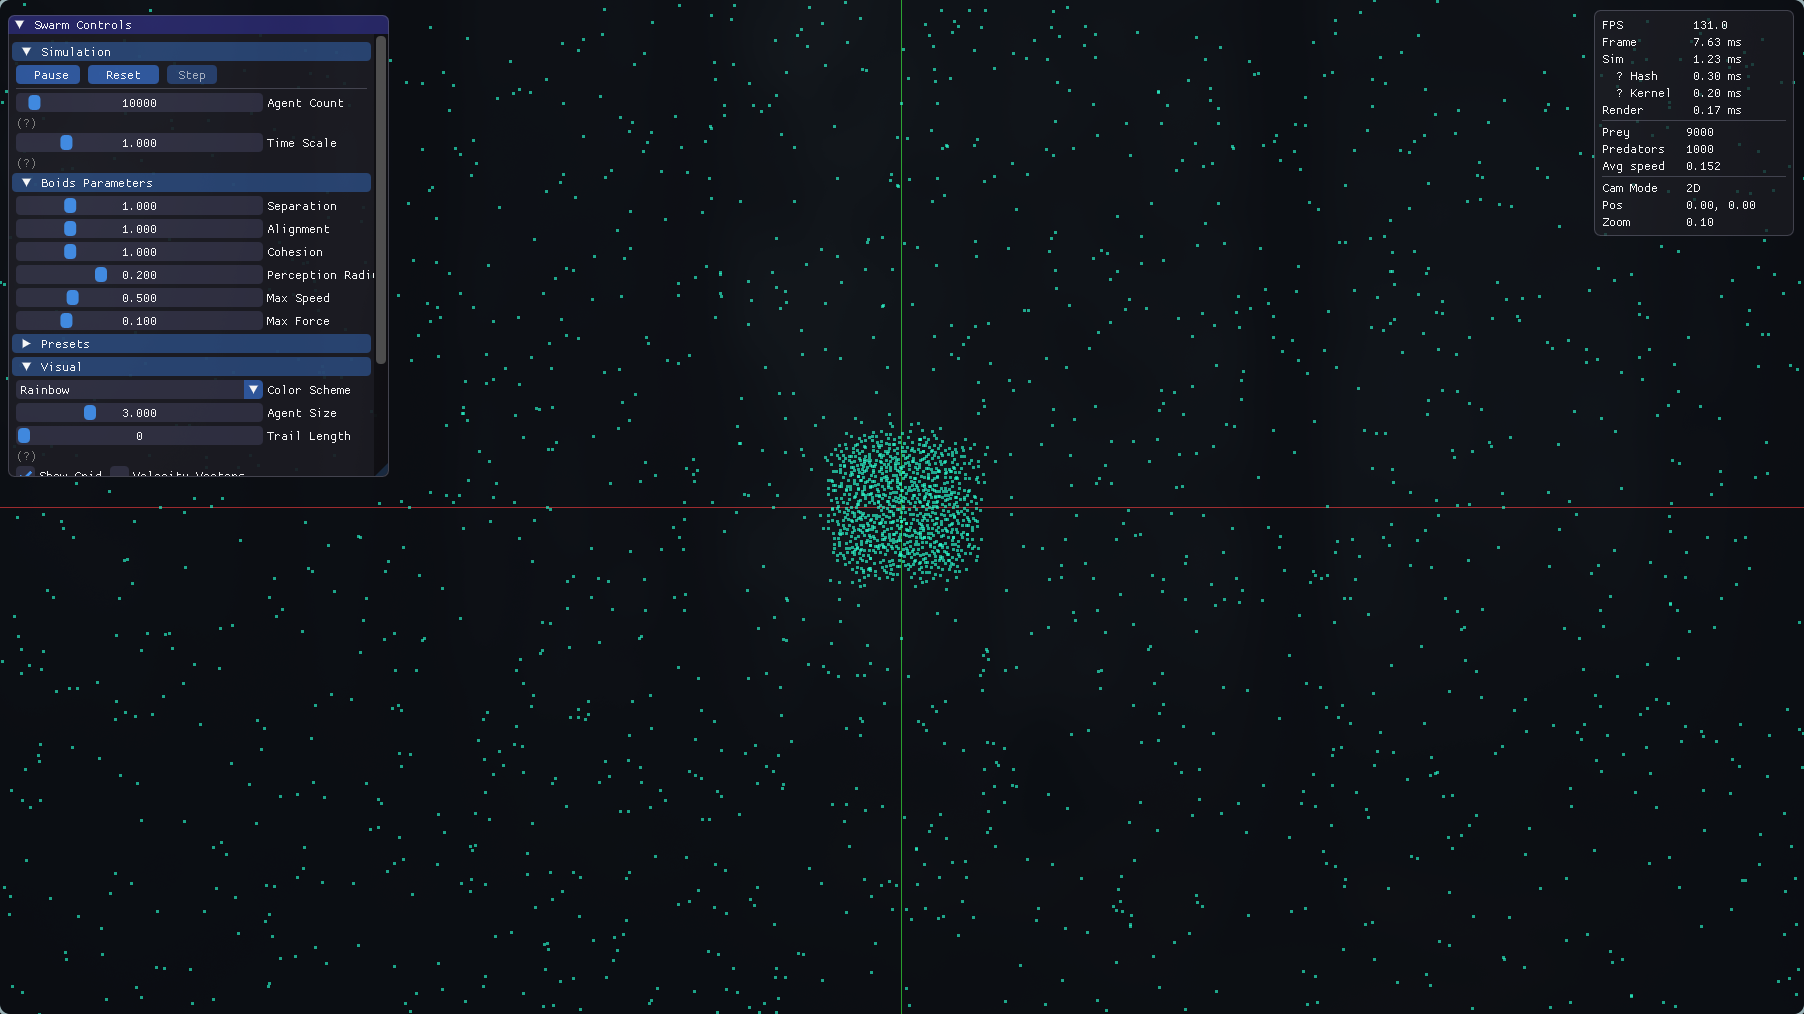
\includegraphics[width=\linewidth]{../images/visual mode-rainbow.png}
        \small Rainbow Mode
    \end{minipage}
    \caption{Comparison of the four distinct shader visualization modes supported by the rendering pipeline.}
    \label{fig:visual_modes}
\end{figure}

\chapter{Performance Evaluation and Benchmarking}

\section{Hardware and Testing Methodology}
To validate the scalability of the $O(N \cdot K)$ spatial hashing model against varying tiers of parallel architecture, the simulation was benchmarked across three distinct systems:
\begin{enumerate}
    \item \textbf{Entry-Level / Mobile:} NVIDIA GeForce MX130
    \item \textbf{Mid-Range Desktop:} NVIDIA GeForce RTX 3050
    \item \textbf{Current-Gen Desktop:} NVIDIA GeForce RTX 4060
\end{enumerate}
All tests were executed at a fixed 1080p resolution in 2D Orthographic mode with the \textit{Velocity Heat-map} shader active.

\section{Scalability Analysis (FPS vs. Agent Count)}
The primary metric for real-time simulation is maintaining a framerate above the 60 Hz display threshold. As shown in Figure \ref{fig:scalability_graph}, the $O(N \cdot K)$ complexity allows even an entry-level MX130 to maintain $>60$ FPS up to 70,000 agents. The RTX 4060 demonstrates massive throughput, rendering 100,000 agents at 470 FPS.

\begin{figure}[H]
    \centering
    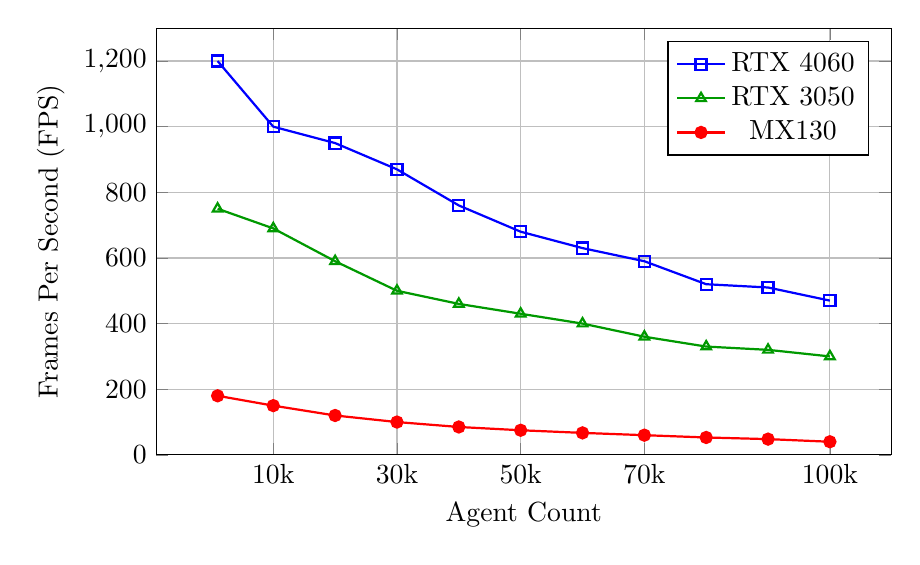
\begin{tikzpicture}
    \begin{axis}[
        width=0.9\textwidth,
        height=7cm,
        xlabel={Agent Count},
        ylabel={Frames Per Second (FPS)},
        grid=major,
        legend pos=north east,
        scaled x ticks=false,
        xtick={10000, 30000, 50000, 70000, 100000},
        xticklabels={10k, 30k, 50k, 70k, 100k},
        ymin=0, ymax=1300
    ]
    % RTX 4060
    \addplot[color=blue, mark=square, thick] coordinates {
        (1000,1200) (10000,1000) (20000,950) (30000,870) (40000,760) (50000,680) 
        (60000,630) (70000,590) (80000,520) (90000,510) (100000,470)
    };
    \addlegendentry{RTX 4060}
    % RTX 3050
    \addplot[color=green!60!black, mark=triangle, thick] coordinates {
        (1000,750) (10000,690) (20000,590) (30000,500) (40000,460) (50000,430) 
        (60000,400) (70000,360) (80000,330) (90000,320) (100000,300)
    };
    \addlegendentry{RTX 3050}
    % MX 130
    \addplot[color=red, mark=*, thick] coordinates {
        (1000,180) (10000,150) (20000,120) (30000,100) (40000,85) (50000,75) 
        (60000,67) (70000,60) (80000,53) (90000,48) (100000,40)
    };
    \addlegendentry{MX130}
    \end{axis}
    \end{tikzpicture}
    \caption{Hardware scalability comparison showing FPS decay as agent count increases from 1,000 to 100,000.}
    \label{fig:scalability_graph}
\end{figure}

\section{CUDA Execution Profiling and Bottleneck Identification}
To capture empirical execution metrics without relying on external profiling software (like NVIDIA Nsight), the simulation integrates native hardware timers directly into the C++ simulation loop using the \texttt{cudaEventRecord} API. This ensures millisecond-accurate timing of the GPU kernels without stalling the CPU thread. These live diagnostic metrics—including the Thrust Radix Sort execution time and the Physics Integration Kernel time—are actively streamed back to the host and rendered in real-time on the Dear ImGui Performance Overlay. 

While the overall framerate scales exceptionally well, this deep profiling uncovers the exact point of hardware saturation. The data visualized below was captured dynamically from the UI overlay on the MX130 to exaggerate the bottleneck conditions. 

\begin{figure}[H]
    \centering
    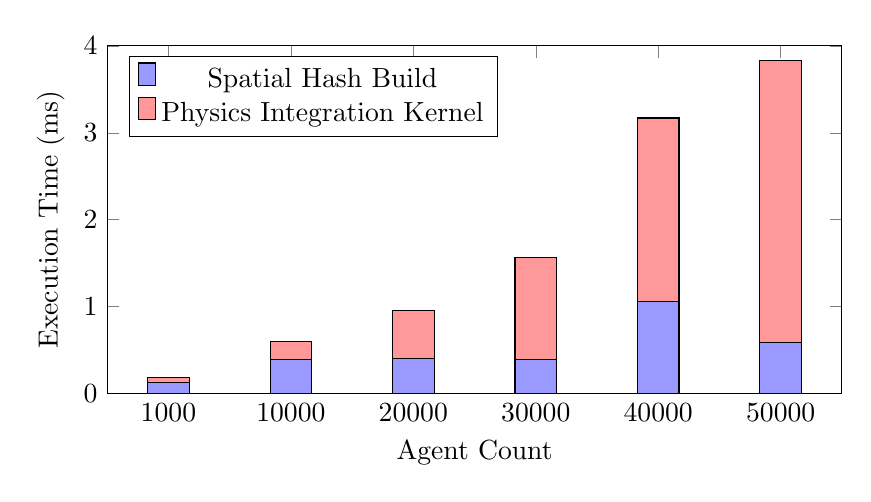
\begin{tikzpicture}
    \begin{axis}[
        ybar stacked,
        width=0.9\textwidth,
        height=6cm,
        bar width=15pt,
        xlabel={Agent Count},
        ylabel={Execution Time (ms)},
        ymin=0, ymax=4.0,
        xtick=data,
        symbolic x coords={1000, 10000, 20000, 30000, 40000, 50000},
        legend pos=north west
    ]
    % Hash Build Time
    \addplot[fill=blue!40] coordinates {
        (1000,0.13) (10000,0.39) (20000,0.41) (30000,0.39) (40000,1.06) (50000,0.59)
    };
    \addlegendentry{Spatial Hash Build}
    % Physics Kernel Time
    \addplot[fill=red!40] coordinates {
        (1000,0.06) (10000,0.21) (20000,0.55) (30000,1.18) (40000,2.11) (50000,3.24)
    };
    \addlegendentry{Physics Integration Kernel}
    \end{axis}
    \end{tikzpicture}
    \caption{CUDA Pipeline breakdown on the MX130. The Physics Kernel execution time aggressively overtakes the Spatial Hashing time beyond 30,000 agents due to the exponential rise in grid cell occupancy queries.}
    \label{fig:profiling_graph}
\end{figure}

As visualized in Figure \ref{fig:profiling_graph}, at lower counts (1k-10k), the overhead of Thrust Radix Sorting the Spatial Hash actually outweighs the Physics Kernel integration. However, as density increases towards 50,000 agents, grid cells become heavily congested. Consequently, the constant $O(K)$ neighbors queried per agent begins to grow substantially, resulting in the Physics Integration step ballooning to $3.24$ ms and dominating the pipeline's execution time.

\chapter{User Interface and Interactive Ecosystem}

\section{Dear ImGui Integration}
The application features a robust real-time diagnostic and control interface powered by Dear ImGui. Because the simulation operates asynchronously via the CUDA default stream, ImGui runs entirely on the CPU thread, submitting draw commands independently of the physics workload. 

The interface is logically partitioned into functional tabs, providing absolute control over the simulation parameters:
\begin{itemize}
    \item \textbf{Steering Weights:} Sliders to adjust the Separation, Alignment, and Cohesion forces in real-time.
    \item \textbf{Kinematics:} Tuning maximum speed, maximum force, and perception radii.
    \item \textbf{Environment:} Injecting global wind vectors, placing mouse-driven attractors, and spawning arbitrary obstacles dynamically.
    \item \textbf{Predator-Prey Ecosystem:} Adjustments for the \textit{Predator Ratio} (which schedules a safe spatial re-initialization), \textit{Predator Speed Multiplier}, and \textit{Fear Weight}. Furthermore, the interface supports real-time manipulation of the ecosystem state; users can trigger \texttt{addAgent(PREDATOR)} or \texttt{convertRandomAgent()} to inject or mutate individual agents live, directly interfacing with the GPU device memory without halting the continuous CUDA physics stream.
\end{itemize}

\section{Visual Tab and Rendering Overrides}
Beyond physical parameters, the UI exposes a "Visuals" tab, directly interfacing with the \texttt{RenderOptions} struct sent to the OpenGL pipeline each frame:
\begin{itemize}
    \item \textbf{Color Schemes:} Users can toggle between four distinct shading models:
    \begin{itemize}
        \item \textit{Uniform:} A solid, single color for all agents to maximize rendering performance.
        \item \textit{Velocity Heat-map:} A dynamic gradient mapping an agent's current speed (velocity magnitude) to color, providing immediate visual feedback on kinetic energy.
        \item \textit{Type (Prey/Predator):} A binary color mapping distinguishing between \texttt{PREY} and \texttt{PREDATOR} agent types, crucial for observing ecosystem dynamics.
        \item \textit{Rainbow:} An aesthetic spatial gradient that maps world-space coordinates or agent IDs to a full RGB spectrum.
    \end{itemize}
    \item \textbf{Agent Geometry:} Sliders to manipulate global \textit{Agent Size}, allowing for clearer visualization at macro scales.
    \item \textbf{Diagnostic Overlays:} Toggles to display individual \textit{Velocity Vectors} as debug lines, or to \textit{Show Grid} to visualize the underlying spatial hashing partitions.
    \item \textbf{Trail Dynamics:} Controls to adjust the maximum \textit{Trail Length} and alpha decay rates, critical for maintaining high frame rates while still visualizing historical swarm trajectories.
\end{itemize}

\begin{figure}[htbp]
    \centering
    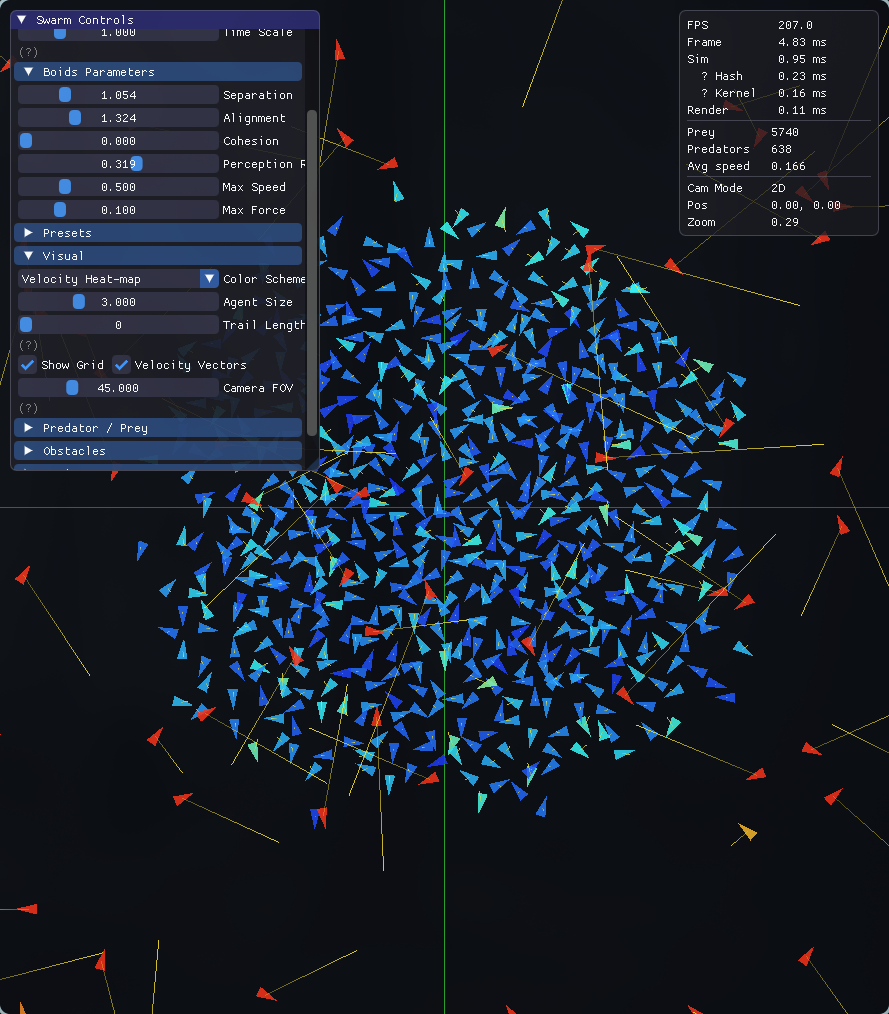
\includegraphics[width=0.85\textwidth]{../images/grid and velocity vectors.png}
    \caption{The real-time ImGui diagnostic overlay. Displaying the individual \textit{Velocity Vectors} and the underlying \textit{Spatial Hashing Grid} directly inside the visualization pipeline.}
    \label{fig:ui_overlay}
\end{figure}

\section{State Management, Exporting, and Recording}
To facilitate structured demonstration, reproducible research, and media generation, the UI implements a comprehensive serialization and output engine:
\begin{itemize}
    \item \textbf{Scenario and Preset Serialization:} Users can construct specific parameter sets (e.g., "Tight Murmuration", "Predator Evasion") and append the \texttt{SimParams} struct to \texttt{config/presets.json} via the "Export Params" feature. A scenario orchestration system allows for scripted narrative demonstrations over a defined timeline.
    \item \textbf{Full State Export/Load:} Beyond simple parameters, the "Export State" functionality serializes the entire simulation context—including \texttt{RenderOptions} and the exact placement and velocities of all dynamic obstacles—into a comprehensive JSON file. "Load State" fully reconstructs this ecosystem and triggers a re-initialization.
    \item \textbf{High-Fidelity Media Capture:} Researchers can capture the visual output asynchronously. "Screenshot" extracts the current OpenGL framebuffer to a PNG in the \texttt{screenshots/} directory. "Start Recording" initiates a sequential frame-dump to the \texttt{frames/} directory, allowing the generation of uncompressed 60FPS video using external tools like FFmpeg without tying the simulation logic to a video encoder's latency.
\end{itemize}

\section{Scripted Scenarios and Orchestration}
Beyond static presets, the engine features a temporal orchestration system (\texttt{scenarios.cpp}) capable of manipulating parameters over time to demonstrate complex emergent phenomena. Four distinct scenarios are natively supported:
\begin{enumerate}
    \item \textbf{Murmuration:} Spawns 15,000 agents with high alignment and dynamic, oscillating wind vectors to simulate sweeping avian flight patterns.
    \item \textbf{Predator Attack:} Spawns 10,000 agents with a 5\% predator ratio. At exactly $T=5.0s$, the "Fear Weight" parameter spikes globally to 8.0f, inducing a dramatic, synchronized radial scatter event.
    \item \textbf{Obstacle Course:} Spawns 8,000 agents navigating a field of static circular obstacles. At $T=10.0s$, the static obstacles suddenly acquire random velocity vectors, forcing the swarm to adapt to a dynamic, chaotic environment.
    \item \textbf{Migration:} Spawns 12,000 agents reacting to a high-strength global attractor. The attractor's coordinates continuously shift across the simulation boundary, forcing the swarm to organize into trailing migratory columns.
\end{enumerate}

\chapter{Future Work and Extensions}
While the current architecture represents a highly optimized 2D simulation, several avenues remain for expansion:

\section{Three-Dimensional Volumetric Simulation}
The most direct extension is expanding the 2D Cartesian plane into a 3D volumetric space. This requires transitioning the spatial hash function from a 2-tuple $(cx, cy)$ to a 3-tuple $(cx, cy, cz)$, recalculating boundary interactions, and upgrading the rendering pipeline to handle depth buffering and projective 3D camera matrices.

\section{Multi-GPU Peer-to-Peer Execution}
For simulations exceeding 1 million agents, a single GPU's VRAM and streaming multiprocessors become insufficient. Utilizing NVIDIA's NVLink interconnect, the uniform spatial grid could be dynamically partitioned. By allocating the left hemisphere to GPU0 and the right to GPU1, only agents located near the spatial meridian would require cross-device peer-to-peer memory access, massively scaling the simulation ceiling.

\section{Machine Learning Driven Behaviors}
Currently, the weights for separation, alignment, and cohesion are statically defined by the user. By integrating a deep reinforcement learning framework (such as TensorRT), agents could actively mutate their weights using evolutionary algorithms. Fitness functions could be designed to reward minimal energy expenditure or maximum predator evasion duration, allowing the simulation to autonomously discover optimal biological flocking parameters.

\chapter{Conclusion}
This project successfully demonstrates the immense computational superiority of GPGPU architectures in simulating complex, emergent biological systems. By translating the mathematically simplistic but computationally heavy $O(N^2)$ Boids algorithm into an optimized $O(N \cdot K)$ CUDA implementation, the historical limits of CPU-bound agent simulations have been shattered. 

The synthesis of highly optimized data structures—namely uniform grid spatial hashing and parallel radix sorting—with low-level hardware interoperability (zero-copy VBO sharing) yields a system capable of modeling 200,000 distinct entities at interactive frame rates. The resulting real-time visualization not only serves as a mesmerizing display of emergent complexity but also stands as a robust educational framework demonstrating the practical application of parallel computing principles, memory coalescing, and graphics pipeline optimization.

\renewcommand{\bibname}{References}
\begin{thebibliography}{99}

\bibitem{reynolds} 
Reynolds, C. W. (1987). 
\textit{Flocks, herds and schools: A distributed behavioral model}. 
ACM SIGGRAPH Computer Graphics, 21(4), 25-34.

\bibitem{cuda_guide} 
NVIDIA Corporation. (2023). 
\textit{CUDA C++ Programming Guide}.

\bibitem{green}
Green, S. (2008). 
\textit{Particle Simulation using CUDA}. 
NVIDIA Developer Technology.

\bibitem{opengl_spec} 
Khronos Group. (2021). 
\textit{OpenGL Registry and Specifications}.

\bibitem{thrust}
Hoberock, J., \& Bell, N. (2010).
\textit{Thrust: A Parallel Template Library}.

\bibitem{tu}
Tu, X., \& Terzopoulos, D. (1994).
\textit{Artificial fishes: Physics, locomotion, perception, behavior}.
Proceedings of the 21st annual conference on Computer graphics and interactive techniques, 43-50.

\end{thebibliography}

\end{document}
